\section{Networks-On-Chip}\label{sec:networkonchip}
\textit{Networks-on-Chip} (or \textit{\glspl{noc}} for short) are a method of interconnecting components on a chip. Typically employed on
\textit{Multi-Processor Systems-on-Chip (\glspl{mpsoc})} \cites(e.g.)(){ivanov05nocintroduction}{biswas15routerattack}{tatas16designingnocs}, they
provide the communication infrastructure for \textit{processing elements (\glspl{pe})} and possibly other \gls{ip} cores.

The topology of a \gls{noc} can vary. Researchers usually assume a 2D mesh topology (cites here), which will also be used throughout this thesis.
% TODO: find a paper where a non-2D-mesh topology is used
In this case, each network node is connected to its four neighbors (excluding the boundary nodes).

A node typically consists of a processing element, a network interface (\textit{\gls{ni}}), and a router. (e.g. cites here). The router manages the connections to
neighboring nodes while also allowing the local processing element to communicate with the network through the network interface. An example of this
architecture is given in Figure \vref{fig:nocexample}.

In a \gls{noc} architecture, each processing element has a \textit{network interface (\gls{ni})}. This interface connects the processing element to a
router. The actual network is established between all

Compared to traditional bus-based interconnect systems, \glspl{noc} can provide a lot of advantages, especially for many-core systems.
\cite[5\psqq]{tatas16designingnocs} One big advantage is scalability; because the cores do not share a global bus, \enquote{local performance is not
degraded} \cite[6]{tatas16designingnocs} as more components are added, and \enquote{aggregated bandwidth scales with the network size}
\cite[6]{tatas16designingnocs}.

In addition, the absence of global connections facilitates the use of different clock domains. This enables the implementation of the
\textit{globally asynchronous, locally synchronous (\gls{gals})} paradigm, which becomes increasingly important in chip design.
\cites[3]{kumar02networkonchip}[2]{ivanov05nocintroduction}

Furthermore, with the constantly increasing design complexity of modern chips \cite{mack11mooreslaw}, specialized on-chip
interconnections become infeasible to implement. Designing such a system \enquote{would take too much time and mapping of applications to dedicated
architectures would be impossible} \cite[1]{kumar02networkonchip}. In contrast, \glspl{noc} aims to be general purpose interconnect systems; they
\enquote{facilitate […] modularity by defining a standard interface} \cite[1]{dally01routepacketsnotwires}.

\begin{figure}
    \centering
    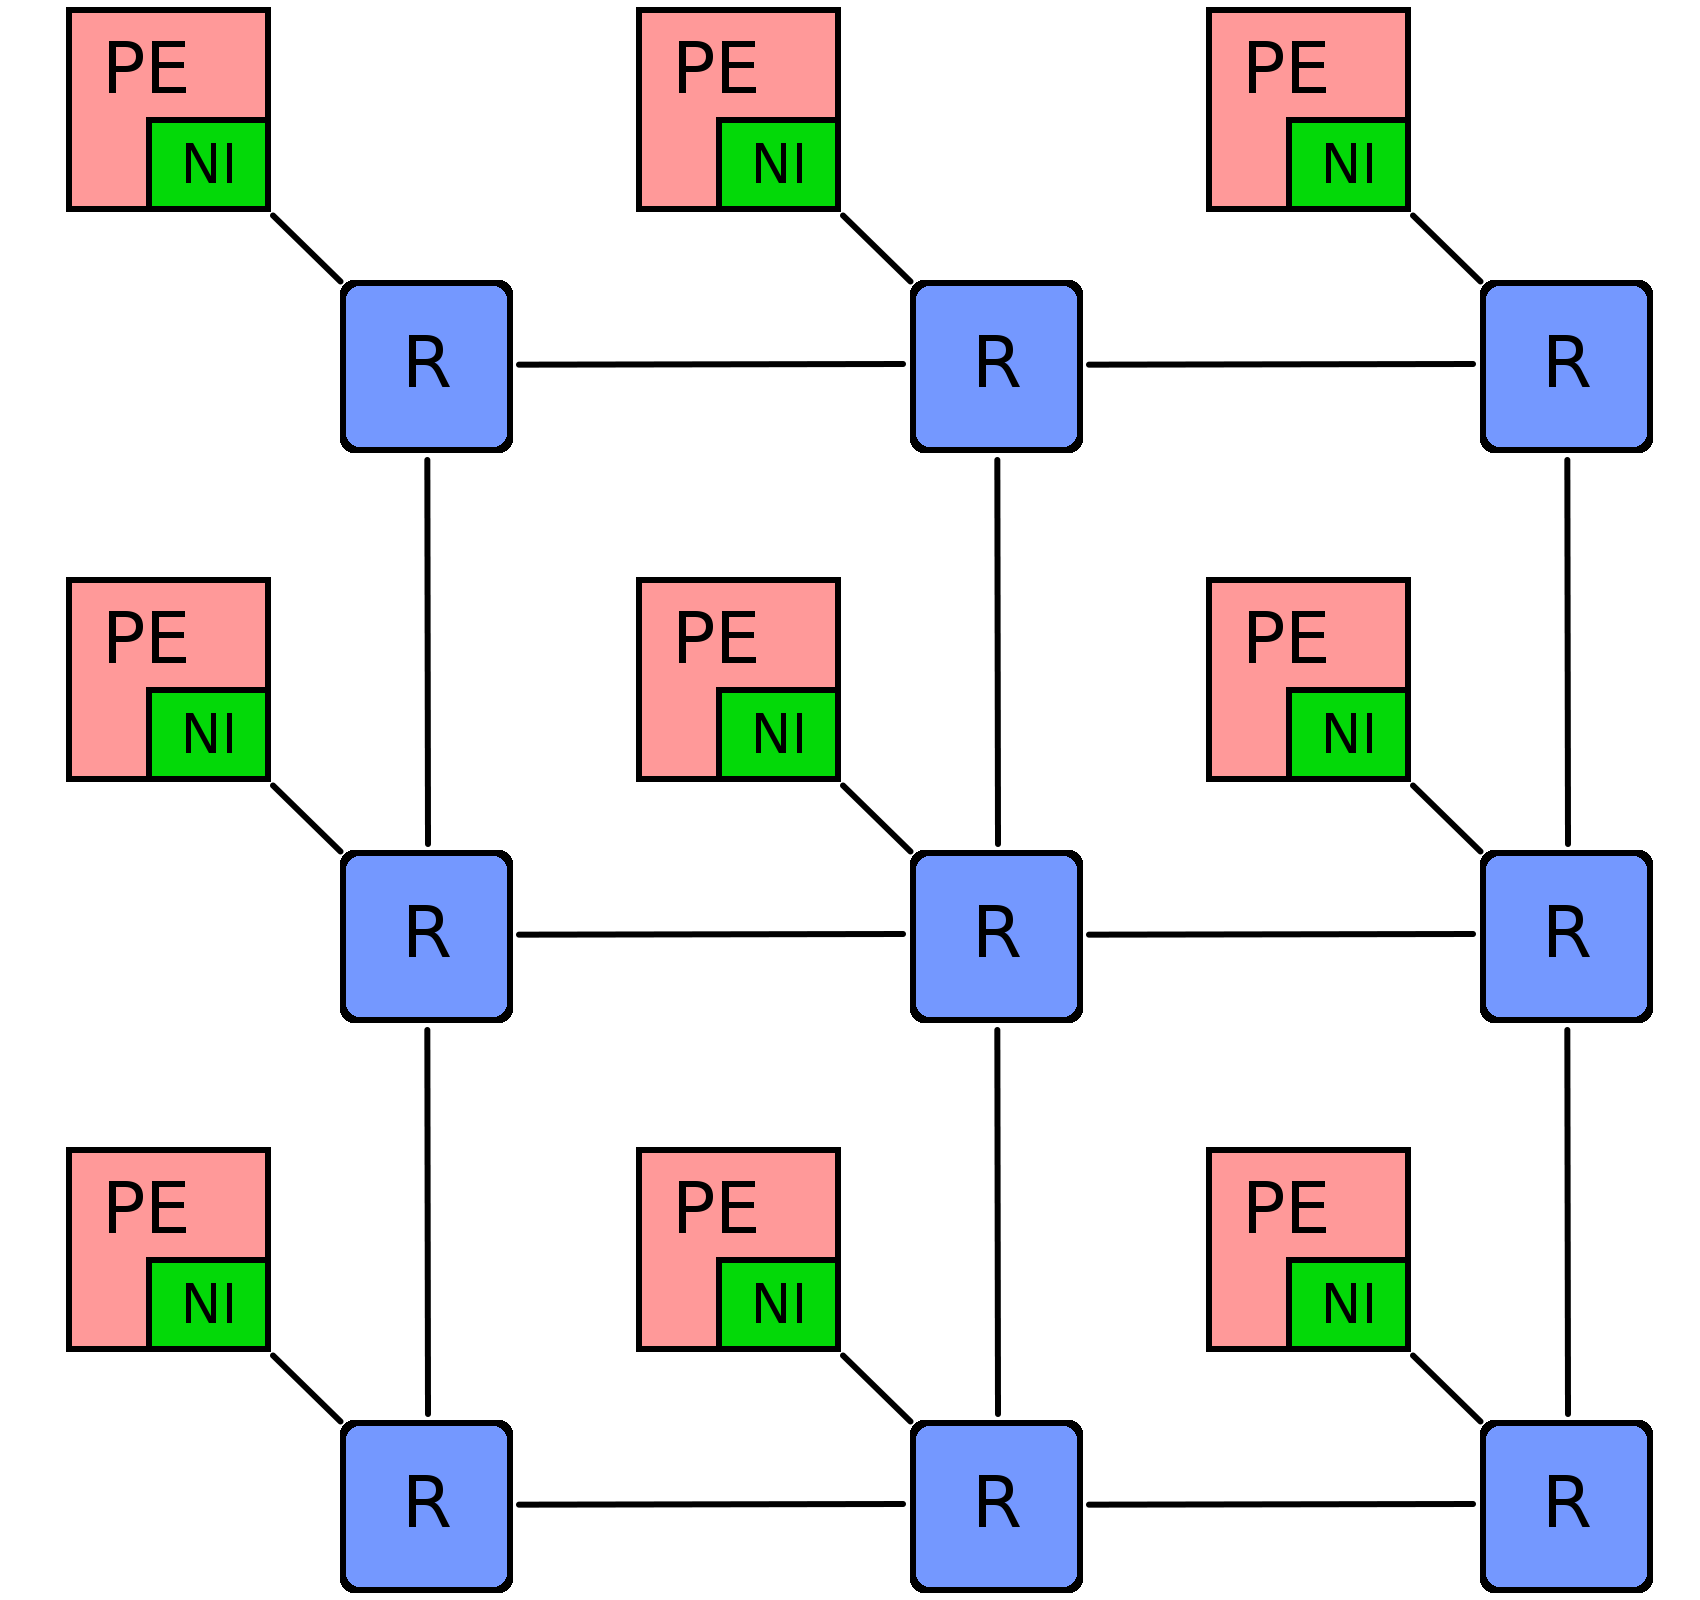
\includegraphics[width=0.5\textwidth]{noc_3x3_colored}
    \caption[Short text]{Long text} % TODO: caption
    \label{fig:nocexample}
\end{figure}

\section{Hardware Trojans}\label{sec:hardwaretrojans}

